\documentclass[journal]{IEEEtran}

\usepackage[utf8]{inputenc}
\usepackage[T1]{fontenc}
\usepackage{graphicx}
\usepackage{booktabs}
\usepackage{amsmath,amssymb}
\usepackage{balance}
\usepackage{cite}
\usepackage{url}

\newcommand{\aliasname}{coherent-offset alias}

\begin{document}

\title{Coherent-Offset Aliasing in UAV-to-Satellite Geo-Localization:\\ Taxonomy, Measurement, and Why Consistency-Based Rejection Fails}

\author{Prabhat~Pandey\thanks{Manuscript submitted for review. Companion materials, per-frame artifacts, and the pre-registered replication protocol accompany this work.}}

\markboth{Draft v6}{COHERENT-OFFSET ALIASING IN UAV-TO-SATELLITE GEO-LOCALIZATION}

\maketitle

\begin{abstract}
UAV geo-localization against satellite reference imagery fails on repetitive terrain in ways standard robustness tools cannot see. We characterize the failure on UAV-VisLoc and separate it into two classes: \emph{whole-tile} aliases, where the matcher locks onto a look-alike tile hundreds of metres away, and \emph{sub-tile} aliases, where the match lands on the correct tile but displaced by one period of a repeating structure invisible at satellite resolution. Three measurements make the case. First, signed per-frame offsets ($n=610$ contiguous frames) show that magnitude histograms---the standard reporting convention---hide the alias class's bimodality and its hole at zero. Second, a benchmark of four published rejection designs over one accepted-fix stream shows that sequential consistency and ORB-SLAM's three-keyframe rule discriminate \emph{backwards} on the sub-tile class (retaining wrong fixes at a higher rate than correct ones), while pairwise consistency and robust frame alignment discriminate forward only by keeping 7--40\% of correct fixes; no consistency-based method meets a pre-registered adoption bar, whereas a prior-ratio gate separates the whole-tile class completely (0 of 7 fatal fixes kept per drift at 150\,m and 300\,m). Third, the alias offset is temporally coherent (2.55$\times$ below a shuffled null at lag 1)---which is exactly why consistency fails---and the mechanism-motivated countermeasure, a multi-hypothesis mixture filter, recovers none of the oracle gap because the alias lattice is per-field and unobservable in the satellite texture. The signature and rate structure reproduce under three further matchers (ORB, SIFT, SuperPoint+LightGlue); a dense matcher (RoMa) adds a third failure mode---a globally smooth, confident warp displaced 55\,m--11\,km---while the same family reports 15\,m at 95\% on contemporary matched-modal imagery, showing published dense-matcher accuracies presume modal proximity. Ten-match averaging cuts the pooled median 21.8 to 8.0\,m---except on whole-tile terrain, where short averages first do worse (Finding~12). A spacing-isolation experiment on 429 video-rate frames identifies temporal spacing as the governing variable: geo-registered fix propagation converts 74\% per-frame solvability into 97\% frame coverage at zero accuracy cost, while the identical chain at 250\,m stride collapses to 25\%. A boundary map over all eleven regions, an executed replication on an independent urban dataset (which also exposes a 16.5\,m georeferencing bias), and a pre-registered replication protocol complete the contribution.
\end{abstract}

\begin{IEEEkeywords}
Geo-localization, perceptual aliasing, robust estimation, UAV, satellite imagery, failure analysis.
\end{IEEEkeywords}

\IEEEpeerreviewmaketitle

\section{Introduction}
\IEEEPARstart{G}{PS}-denied UAV navigation increasingly relies on matching nadir drone imagery against georeferenced satellite tiles to anchor drift-prone visual-inertial odometry. Published systems report median errors of metres on favourable terrain~\cite{anyvisloc,orthotrack,ortholoc}. Failure analysis, however, is thin: benchmarks report accuracy at thresholds (A@$X$\,m) over pooled terrain, which is blind to how, where, and why the tail fails. Recent mitigation systems acknowledge aliasing explicitly---trajectory-level VPR fusion~\cite{naviloc}, particle filtering with learned aliasing gates~\cite{cpfl}, correspondence propagation~\cite{orthotrack}---but they assume the temporal-consistency and trusted-odometry regime they need; the behaviour of that regime's rejection tools on the alias classes themselves has not been measured.

We document a failure class on repetitive terrain---farmland with parallel furrows, forest canopy---where accepted matches are wrong by tens to hundreds of metres \emph{with full geometric and appearance support}. We show this class defeats the standard robustness toolbox for a measurable, mechanical reason, we show the failure is not an artifact of any one matcher---sparse or dense---and we quantify what would be required to fix it, including the one regime change (video-rate capture with fix propagation) that measurably contains it.

Coherent (mutually consistent) outliers in SLAM are studied theoretically for indoor scenes~\cite{lajoie2019}; row-level aliasing on vineyard rows is reported from ground robots with LiDAR~\cite{desilva2026,desilva2025,tempovine}. Neither provides cross-view (nadir UAV $\leftrightarrow$ satellite) measurements, per-class rejection behaviour, nor the temporal-coherence and appearance-optimality measurements we report. STHN notes self-similar patterns as a confound in UAV thermal$\leftrightarrow$satellite homography~\cite{sthn} and UASTHN detects such failures via uncertainty estimation~\cite{uasthn}, but neither analyzes the alias structure. Robust pose-graph back-ends (PCM, GNC, TACO) are designed against exactly this outlier shape~\cite{mangelson2018,kimera,yang2020,taco}; we measure how the standard representatives of this family behave on real cross-view data. Learned dense matchers (RoMa, LoFTR, RoMav2) are benchmarked on matched-modal contemporary imagery~\cite{xianvisloc}; we measure the same family on vintage-mismatched pairs and show the benchmark numbers do not transfer---a finding consistent with concurrent work that documents dense-matching unreliability under temporal gaps at remote-sensing scale~\cite{loretta} and adapts RoMa specifically to survive multi-temporal UAV-to-orthophoto pairs~\cite{satroma}.

\noindent\textbf{Contributions.}
\begin{enumerate}
\item \textbf{A taxonomy} separating whole-tile from sub-tile aliases, each with a distinct geometry, temporal signature, and rejection behaviour (Sec.~\ref{sec:structure}, \ref{sec:coherence}).
\item \textbf{Backwards-rate tables} for four published rejection methods over a shared fix stream: sequential consistency and the three-keyframe rule keep wrong fixes at a \emph{higher} rate than correct ones; PCM and robust frame alignment discriminate forward only by destroying 60--93\% of correct fixes; only a prior-normalized distance gate works, and only on the whole-tile class (Sec.~\ref{sec:bench}).
\item \textbf{Matcher independence}: the alias signature and the rate structure reproduce under ORB-only, SIFT-only, and SuperPoint+LightGlue---three correspondence sources spanning binary corners, gradient blobs, and a learned detector--matcher---and dense matchers add a third failure mode with its own mechanism (Sec.~\ref{sec:matcher}).
\item \textbf{The sign-folding diagnostic}: absolute-value error histograms fold symmetric alias structure into an apparently continuous distribution; signed offsets recover the axis and the hole at zero (Sec.~\ref{sec:structure}).
\item \textbf{A falsified countermeasure}: the mixture hedge filter that follows from the mechanism recovers none of the oracle gap, because the alias lattice is per-field and unobservable---with a reproducible oracle bound of 14.0\,m median quantifying the residual (Sec.~\ref{sec:counter}).
\item \textbf{An exhaustive terrain boundary map} over all eleven source-dataset regions plus held-out and cross-dataset controls confirming the class is terrain-specific, and a pre-registered replication protocol (Sec.~\ref{sec:boundary}, \ref{sec:replication}).
\item \textbf{A spacing-isolation measurement} (Sec.~\ref{sec:spacing}): at metre-scale frame spacing, geo-registered fix propagation---the mechanism underlying~\cite{orthotrack,naviloc}---carries one anchored fix for an entire flight at baseline accuracy (74\%$\to$97\% frame coverage, zero accuracy cost); at 250\,m stride the identical chain collapses. Temporal spacing---not the matcher, not the geometry---is the governing variable for fix propagation, with matched-modal controls showing terrain class operates independently of imagery vintage.
\end{enumerate}

\section{Related Work}

\textbf{UAV--satellite geo-localization.} Retrieval-based systems~\cite{uavvisloc,anyvisloc,denseuav} and geometric pipelines (homography, as in the production matcher studied here; PnP against DSM~\cite{ortholoc,orthotrack}) are benchmarked by pooled accuracy-at-threshold. AnyVisLoc's Table~6 is representative: its baseline scores 74.1\% A@5\,m against an aerial photogrammetry reference but 18.5\% A@5\,m against a satellite reference~\cite{anyvisloc}---the satellite-reference tail exists, is large, and is not analyzed per-region. Our work is complementary: we analyze \emph{why} that tail exists rather than improving its head.

\textbf{Perceptual aliasing and robust estimation.} Aliasing in place recognition is a classic concern~\cite{lowry2016}; sequence-based VPR exploits temporal consistency to combat it~\cite{seqvpr}. Modern robust back-ends address mutually consistent outliers with pairwise consistency (PCM~\cite{mangelson2018}, Kimera-RPGO~\cite{kimera}), graduated non-convexity (GNC~\cite{yang2020}), or robust kernels on pose-graph factors (TACO~\cite{taco}). Lajoie et al.\ analyze coherent outliers in indoor SLAM theoretically and note that mutually consistent outliers defeat initial-guess-dependent rejection~\cite{lajoie2019}. Vineyard robotics reports row-level aliasing from ground LiDAR qualitatively~\cite{desilva2025,desilva2026,vineptmap}. Multi-hypothesis handling of aliasing dates to hypothesize-and-verify loop closure~\cite{tanaka2016}. None of these measures the rejection \emph{rate} of published methods on a shared cross-view fix stream, nor the temporal coherence of the alias offset itself---the measurements we contribute.

\textbf{Systems that assume the answer.} A 2026 generation of deployed-system work builds the mitigation layer whose assumptions we test. NaviLoc~\cite{naviloc} fuses per-frame VPR with VIO through a three-stage trajectory estimator (global SE(2) alignment, sliding-window Procrustes refinement, convex MAP smoothing with outlier clamping), reporting 19.5\,m mean error on a rural benchmark at 9\,FPS on an embedded board---its design presumes video-rate trusted relative motion and treatable VPR outliers. CPFL~\cite{cpfl} runs a vision-only particle filter whose dual-granularity gating is explicitly designed ``to mitigate perceptual aliasing,'' and contributes a Trajectory Continuity Index for continuous localization---an independent sign that the field's pooled per-frame metrics are felt to be insufficient (our signed-offset diagnostic and truth-correlation guard address the same reporting gap at the measurement level). OrthoTrack~\cite{orthotrack} propagates map-anchored correspondences to intermediate frames with optical flow---the chain architecture our Sec.~\ref{sec:chain} instantiates---and SeqLoc~\cite{seqloc} aggregates sequential belief volumes for feature-sparse cross-view localization. All four operate in, or implicitly assume, the video-rate regime; none isolates frame spacing as a variable, and none measures rejection behaviour on coherent aliases. Our spacing-isolation pair (Sec.~\ref{sec:spacing}) and backwards-rate tables (Sec.~\ref{sec:bench}) are the controlled measurements underneath this system family: they say when the assumed regime is necessary (250\,m stride collapses the identical chain) and which of its rejection tools carry aliasing risk (consistency filters fail backwards; prior-ratio gates the separable class).

\textbf{Error distribution analysis in VPR.} Reporting conventions use magnitude histograms and CDFs; CPFL's continuity index is a trajectory-level addition. We show a class of symmetric bimodal error---the signature of period-quantized aliasing---is invisible in magnitude form, and propose signed-offset reporting as a diagnostic (Sec.~\ref{sec:structure}).

\textbf{Matcher dependence of failure rates.} Failure analyses of matching pipelines are usually reported for the authors' own matcher; whether the reported tail is a property of the terrain or of the descriptor pipeline is rarely tested. We test it directly (Sec.~\ref{sec:matcher}): the alias signature is reproduced by every matcher family we can run, and the rejection-rate structure is stable in sign and magnitude across the classical matchers, with the learned matcher underpowered for rates but consistent at the signature level. Dense matchers (RoMa~\cite{roma}, RoMav2~\cite{xianvisloc}) report the strongest fine-localization numbers in the field; we show those numbers presume contemporary matched-modal imagery and that the family adds a distinct failure mode under vintage-mismatch. Concurrent work corroborates the regime dependence from the construction side: LoRetta~\cite{loretta} reformulates dense matching as localization-and-registration precisely because ``intrinsically unmatchable regions make direct dense correspondence prediction unreliable'' across acquisition-time and season gaps, and Sat-RoMa~\cite{satroma} re-engineers RoMa with a satellite-tuned DINOv3 encoder to survive multi-temporal UAV-to-orthophoto pairs. Both build around the failure our Sec.~\ref{sec:matcher} isolates mechanistically in the stock models; neither characterizes the failure mode itself.

\textbf{Fix propagation and odometry regimes.} Tracking geo-registered control points between matched frames so that absolute matching becomes a rare re-anchor rather than a per-frame duty is standard in fielded systems~\cite{yao2024,orthotrack}. Whether the technique survives coarse frame spacing has not been isolated as a variable; the spacing-isolation experiment in Sec.~\ref{sec:spacing} is the first controlled measurement of the regime boundary for geometric fix propagation (SeqLoc's sequence aggregation is the retrieval-side analogue and reports the same single-frame collapse qualitatively).

\section{Method}

\subsection{System under study}
The pipeline is a production map matcher: ORB+AKAZE+SIFT pooled correspondences, MAGSAC homography~\cite{magsac}, image-centre projection through the inverse homography, patch-wide NCC verification at 0.30, \texttt{min\_inliers}=10, DEM-corrected AGL scale. Candidate generation is prior-centred ($5\times5$ tile ring). Frames carry a drifted prior injected as a random walk at 150/300/600\,m. Dataset: UAV-VisLoc~\cite{uavvisloc}, eleven Chinese sites; all measurements use the dataset's drone GPS as truth.

\begin{figure}[t]
\centering

\includegraphics[width=\columnwidth]{figs/fig4_pipeline.png}
\caption{The production map matcher under study and the measurement harness around it. Pooled ORB+AKAZE+SIFT correspondences feed a MAGSAC homography against a prior-centred satellite tile ring; accepted fixes carry the estimate, the prior, and the filter-reported uncertainty that the rejection benchmark consumes.}
\label{fig:pipeline}
\end{figure}

\subsection{Measurement protocol and definitions}
\textbf{Error classes.} A fix is \emph{good} if its error against the dataset GPS is $<$20\,m, \emph{mid} if 20--50\,m, and \emph{fatal} if $\geq$50\,m. These boundaries are fixed a priori and used across all experiments.

\textbf{Signed offsets.} For each frame, we match against the ground-truth tile and record the signed (north, east) offset between the recovered position and the dataset's GPS record. Frames are \emph{contiguous} in flight order ($n=610$ solved on R04 out of 738 attempted), because step-sampling destroys the temporal structure the coherence question needs.

\textbf{Fix stream.} For rejection benchmarks, we run the production matcher under injected drift and keep every accepted fix with its estimate, prior, and prior uncertainty ($n=40$ per region per drift, seed fixed).

\textbf{Metrics.} Good-kept\% / fatal-kept\% with denominators inline; discrimination ratio $=$ good-kept/fatal-kept ($>$1 $=$ forward discrimination). Adoption bar for a rejector: fatal cut $\geq$25\% while keeping $\geq$80\% of good fixes (pre-registered before any benchmark ran).

\subsection{The rejector benchmark}
Four published designs are implemented over the shared fix stream, using only deployed signals (priors, estimates, filter-reported uncertainty): sequential consistency (a fix survives if a neighbouring fix agrees within a motion-compensated tolerance; the ORB-SLAM3 covisibility principle~\cite{orbslam3}), ORB-SLAM's three-consecutive-keyframe rule~\cite{orbslam}, PCM-style greedy maximum clique~\cite{mangelson2018}, and VINS-Mono-style robust frame alignment (median prior$\leftrightarrow$estimate offset, reject residual $>\tau$)~\cite{vinsmono}. The prior-ratio gate (fix kept iff distance to prior $\leq$ $1.5\times$ the prior's uncertainty) is evaluated in deployed (filter RMS) and oracle (true prior error) forms.

\subsection{Matcher variants}
Every pooled-pipeline measurement has a variant protocol in which only the correspondence source changes, everything else (CLAHE preprocessing, DEM/AGL-corrected GSD rescale, GT tile patch, MAGSAC, thresholds) held identical: \emph{ORB-only} (binary corner descriptors~\cite{rublee2011}), \emph{SIFT-only} (gradient-histogram descriptors~\cite{lowe2004}), and \emph{SuperPoint+LightGlue} (learned detector and matcher~\cite{detone2018,sarlin2023}). Variant streams are analysed separately and never pooled with the production stream (cross-quote rule); the production matcher is the ORB+AKAZE+SIFT pool unless a table states otherwise. The dense variant (Sec.~\ref{sec:matcher}) is RoMa \texttt{roma\_outdoor}~\cite{roma} run on the same GT-tile protocol.

\subsection{The propagation chain}
\label{sec:chain}
A geo-registered fix-propagation chain in the family of OrthoTrack's map-anchored correspondence propagation~\cite{orthotrack}, requiring no camera intrinsics: (i)~\emph{seed}: production pool match on a satellite crop centred at the known position (the flight-start GPS assumption); the seed homography maps drone pixels to map pixels. (ii)~\emph{chain}: KLT optical flow tracks the seed keypoints frame-to-frame; a MAGSAC relative homography is fit on the tracked pairs and composed with the accumulated absolute homography; position $=$ frame centre projected through the composed map. (iii)~\emph{re-anchor}: if tracked points fall below 20, relative inliers below 10, or the propagated position exits a 90\,m safe zone around the reference crop, the chain re-matches on a fresh crop centred at the last fix; on failure the frame coasts (no fix). The chain is evaluated on a video-rate dataset (XIAN-VisLoc~\cite{xianvisloc}, trajectory 16: 429 frames, $490\times490$, 3.8\,m median frame step, Level-19 Google reference at 0.24\,m/px, per-frame GPS) in two arms: dense (stride 1) and coarse (stride 65\,$\approx$250\,m---the source dataset's regime). The chain is deliberately minimal---no intrinsics, no learned components---because the experiment's object is the spacing variable, not the estimator; the contribution over~\cite{orthotrack} is the controlled stride pair, not the architecture.

\section{Experiments}
\label{sec:exp}

\subsection{Error structure: the taxonomy and the sign-folding diagnostic}
\label{sec:structure}

\textbf{Setup.} Signed offsets on GT tiles, R04 ($n=32$ step-sampled for regional statistics; $n=610$ contiguous for the full distribution) and R03 ($n=30/557$) as control. The $n=32$ sample and the $n=610$ stream are \emph{different} samples of the same region; baseline medians therefore differ (32.7\,m on $n=32$, 31.1\,m on $n=610$) and are always quoted with their sample size.

\textbf{Result 1---magnitude histograms hide the alias class.} The signed R04 offsets are axis-aligned and bimodal: axial resultant $R=0.50$ (vs.\ 0.19 control) with the \emph{hole at zero} (6/32 frames within $\pm$10\,m along the dominant axis, vs.\ 14/30 on the control). Folded to magnitudes, this is exactly the ``continuous, no-gap'' distribution that earlier analysis misread as imprecision (Fig.~\ref{fig:signed}).

\begin{figure}[t]
\centering

\includegraphics[width=\columnwidth]{figs/fig1_signed_vs_folded.png}
\caption{The sign-folding diagnostic. Left: signed (north, east) offsets on R04 ($n=610$ contiguous) and R03 (step-sampled). The R04 alias class is axis-aligned with a hole at zero; R03 is unstructured. Right: the same R04 data folded to magnitudes---the standard reporting convention---appears continuous and hides the alias class.}
\label{fig:signed}
\end{figure}

\textbf{Result 2---the axis is per-field, not per-region.} At $n=32$ the offsets split into two orientation groups (bearings 145--193$^{\circ}$ and 279--357$^{\circ}$): the flight crosses fields whose furrow orientation changes. A single-region-axis oracle degrades accordingly: the sub-tile snap oracle (best integer period removed along one axis) falls from $2.39\times$ over a random-axis null at $n=16$ to $1.72\times$ at $n=32$, while its absolute ceiling stays stable (12.0--12.7\,m median against a 32.7\,m baseline). The alias is a lattice structure \emph{per field}.

\textbf{Result 3---the wrong lock is the appearance optimum, unanimously.} At $n=32$, masked patch NCC over displaced homographies selects displacement $k=0$ on 32/32 frames; the oracle displacement recovers 20.4\,m of median error (32.7$\to$12.3\,m). Appearance is not merely uninformative on this class; it is monotone \emph{against} the truth.

\textbf{Result 4---whole-tile aliases are a different class.} On forest (R06), the error distribution is bimodal with a clean 40--150\,m gap: discrete jumps to look-alike tiles 1--2 tile widths along track. Their offsets are coherent across the flight turn, following the aircraft.

\textbf{Result 5---the signature replicates within the flight (split-half).} The contiguous $n=610$ stream split at its midpoint shows the signature independently in both halves: axis 168.1$^{\circ}$ vs.\ 166.6$^{\circ}$, hole-at-zero 0.22 vs.\ 0.14, anisotropy 1.69 vs.\ 2.02, alias-group lag-1 coherence 1.16$\times$ ($n=13$) and 3.16$\times$ ($n=12$) below null, good groups at null. The weaker first-half coherence is consistent with Result 2---a half-flight still spans multiple fields with different axes.

\textbf{Result 6---attitude and imagery vintage do not explain the class.} Two reviewer-grade confounds are ruled out with the dataset's own metadata. (a)~\emph{Camera attitude.} The stream is effectively nadir: 608/610 frames have $|$tilt$| \leq 10^{\circ}$ (median $|$pitch$|$ 1.3$^{\circ}$, max 14.2$^{\circ}$ on R04), and excluding the two tilted frames changes nothing (axis 167.4$^{\circ}$, axial $R$ 0.31, hole-at-zero 0.18, median 31.0\,m on $n=608$). The nadir-point correction hypothesis (error $\approx$ alt$\cdot\tan(\mathrm{tilt})$) was tested and killed: a cross-validated correction over all four sign conventions buys 1.6\,m against a 2\,m bar, and the tilt correlation that motivated it ($+0.44$ with error magnitude) was traced to tilt degrading the homography fit rather than to projection geometry. (b)~\emph{Imagery vintage.} Every region is a single-day flight (R03 2018-10-23, R04 2018-10-24, consecutive days in the same district), so any satellite-vintage gap is identical across the pair---yet R03 is the clean control and R04 carries the class. Sec.~\ref{sec:spacing} adds matched-modal controls showing terrain class operates independently of vintage.

\subsection{The backwards-rate benchmark}
\label{sec:bench}

\textbf{Setup.} Production matcher, regions R03 (control, 0 fatal), R04 (sub-tile), R06 (whole-tile); drifts 150/300/600\,m; 255 pooled accepted fixes. Four rejectors plus two prior-ratio forms.

\begin{table}[t]
\caption{Rejection rates over the shared accepted-fix stream (good-kept\%/fatal-kept\%; discrimination ratio $>$1 is forward). tol=$\tau$=100\,m throughout; prior-ratio threshold $r{=}1.5$; bold cells pass the pre-registered adoption bar (fatal cut $\geq$25\%, good kept $\geq$80\%).}
\label{tab:rates}
\centering
\footnotesize
\begin{tabular}{@{}lccc@{}}
\toprule
Rejector & d150 & d300 & d600 \\
\midrule
Seq.\ consistency & 0.96 (96/100) & 0.84 (84/100) & 0.81 (59/73) \\
3-consecutive & 0.95 & 0.97 & 0.45 ($n{=}3$) \\
PCM max-clique & 3.02 (40/13) & 3.17 (23/7) & 0.79 \\
Frame alignment & 2.09 (56/27) & 2.80 (20/7) & 1.12 \\
Prior-ratio (RMS) & \textbf{2.12} (99/47) & 1.08 & 1.00 \\
Prior-ratio (oracle) & \textbf{2.31} (92/40) & \textbf{1.95} (97/50) & \textbf{1.57} (100/64) \\
\bottomrule
\end{tabular}
\end{table}

\textbf{Finding 1---sequential consistency and the three-keyframe rule discriminate backwards on the sub-tile class.} They keep wrong fixes at a \emph{higher} rate than correct ones at every drift (ratio $\leq$0.97 wherever $n$ permits); at tol=100\,m, 100\% of fatal fixes survive at d150 and d300 (Fig.~\ref{fig:rates}).

\textbf{Finding 2---the forward ratios that do exist are coverage-destroying.} PCM and frame alignment reach ratios of 2--3 at tol=100\,m only by keeping 7--40\% of correct fixes---the purity-for-coverage trade, measured as a rate. No consistency-based method passes the adoption bar in any cell at any drift.

\textbf{Finding 3---the whole-tile class is fully separable, the sub-tile class is invisible, per region.} On R06, the prior-ratio gate with honest uncertainty keeps 100\% of good fixes and 0 of 7 fatal fixes per drift at d150 and d300 (14 fatal fixes pooled over the two drifts). On R04 it scores 0.93--1.00: a 20--80\,m alias is small against a 300\,m prior, so no ratio threshold can see it. On the R03 control, the consistency filters destroy 15--76\% of good fixes---collateral measured, not asserted.

\begin{figure}[t]
\centering
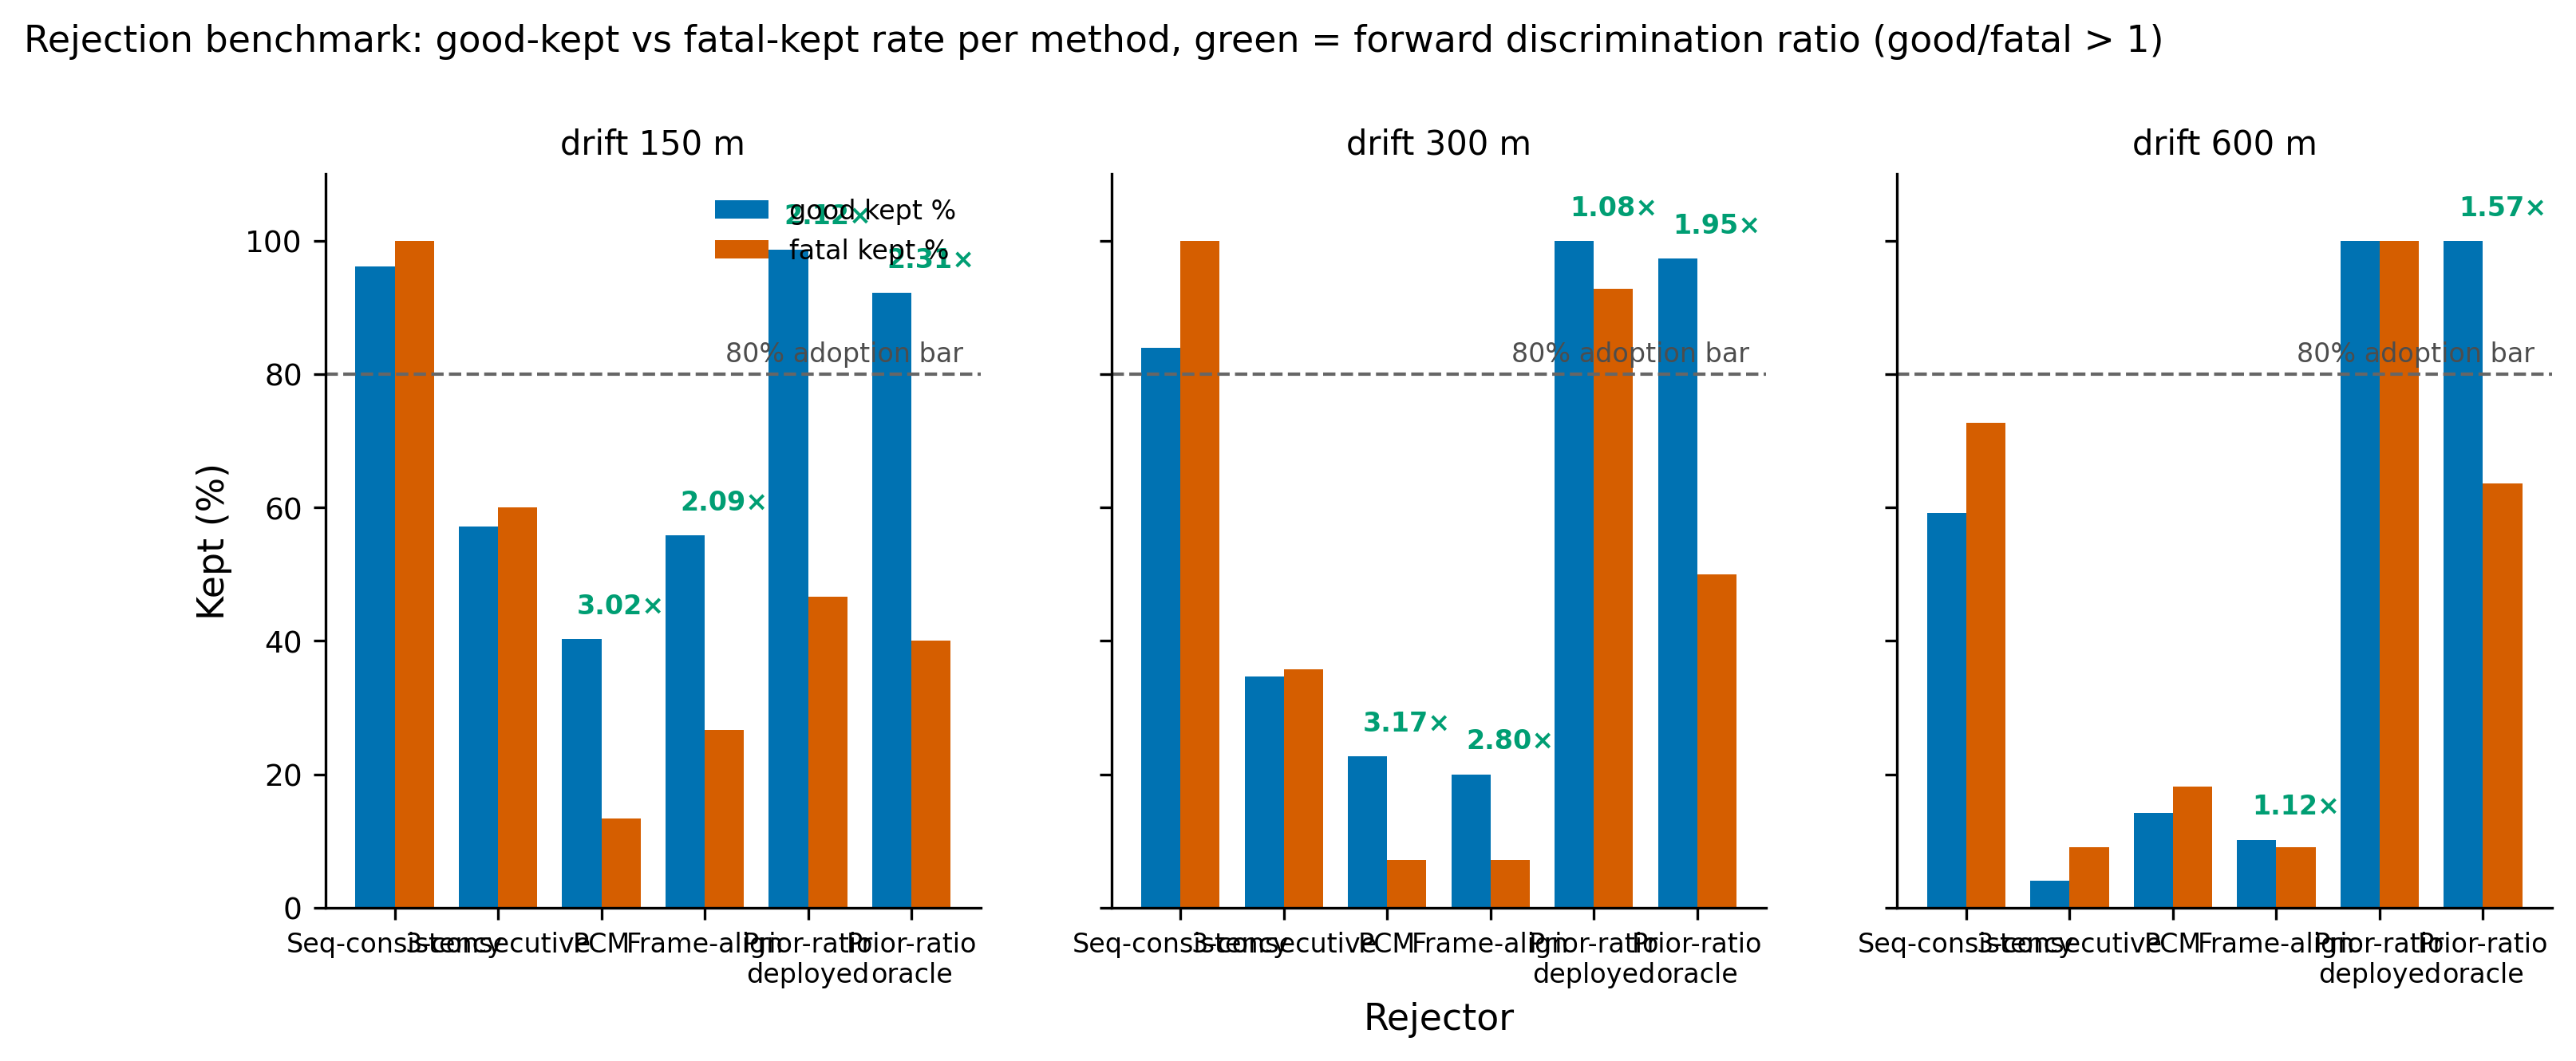
\includegraphics[width=\columnwidth]{figs/fig3_rejector_rates.png}
\caption{Backwards-rate benchmark over the pooled fix stream (255 accepted fixes). Bars: good-kept vs.\ fatal-kept percentage per rejector and drift; dashed line: the 80\% good-kept adoption bar. Sequential consistency and the three-keyframe rule keep fatals at $\geq$ good rates (ratio $\leq$1); PCM and frame alignment score $>$1 only by destroying coverage.}
\label{fig:rates}
\end{figure}

\subsection{Temporal coherence: the mechanism}
\label{sec:coherence}

\textbf{Setup.} Truth-referenced signed offsets, contiguous frames, R04 $n=610$ (alias $\geq$50\,m: 93; mid 20--50\,m: 374; good $<$20\,m: 143), R03 control $n=557$. Per-lag pair counts inline.

\begin{table}[t]
\caption{Median pairwise offset difference vs.\ frame lag (m). Null: offsets shuffled within group (10 trials). $n$ = alias pairs.}
\label{tab:coherence}
\centering
\footnotesize
\begin{tabular}{@{}lccccc@{}}
\toprule
lag & $n$ & alias: med / null & ratio & good: med / null & ratio \\
\midrule
1 & 25 & 27.5 / 70.1 & \textbf{2.55$\times$} & 16.7 / 17.9 & 0.93 \\
2 & 17 & 46.8 / 86.1 & 1.84$\times$ & 15.9 / 17.9 & 0.89 \\
3 & 15 & 27.9 / 63.9 & 2.29$\times$ & 17.2 / 19.3 & 0.89 \\
5 & 12 & 80.0 / 90.1 & 1.13$\times$ & 19.6 / 17.3 & 1.13 \\
8 & 11 & 60.3 / 93.5 & 1.55$\times$ & 14.6 / 18.6 & 0.78 \\
\bottomrule
\end{tabular}
\end{table}

\textbf{Finding 4---the alias offset is locally coherent and decays with lag.} Adjacent alias frames differ by 27.5\,m where random pairing gives 70.1\,m; the advantage decays to $\sim$1.1$\times$ by lag 5--8 (Fig.~\ref{fig:coherence}). The lock is not rigid: it drifts slowly (the period index changes occasionally), coherent over 2--4 frames. Correct fixes are independent per frame (at null at every lag, 0.78--1.13$\times$) and the R03 control matches them. The 20--50\,m band is \emph{partially coherent}---a mixture of alias and noise---which explains why threshold rejectors tuned anywhere in that band fail (Finding 1).

\begin{figure}[t]
\centering

\includegraphics[width=\columnwidth]{figs/fig2_coherence_curve.png}
\caption{Temporal coherence of the alias offset (R04, $n=610$ contiguous). Solid: median pairwise offset difference within the alias ($\geq$50\,m) and good ($<$20\,m) groups; dashed: shuffled nulls. The alias group sits 2.55$\times$ below its null at lag 1 and decays to $\sim$1.1$\times$ by lag 5--8; correct fixes are independent at every lag.}
\label{fig:coherence}
\end{figure}

\textbf{Consequence.} Within the coherence window, an alias chain is exactly as motion-consistent as the truth: pairwise consistency has a gauge symmetry (constant offsets cancel in frame differences), so PCM/sequential consistency are provably blind, not merely weak. Beyond the window, the offset has drifted enough to survive any tolerance that keeps good fixes (their own $\sim$17\,m scatter). The backwards rates of Sec.~\ref{sec:bench} are the statistical image of this geometry.

\subsection{The countermeasure fails for a measured reason}
\label{sec:counter}

\textbf{Setup.} Two routes: (a)~estimate the alias lattice from the map itself---detrended autocorrelation of a 500-px crop around each locked position, strongest local maximum in the 9.5--95\,m band, $n=610$; (b)~a multi-hypothesis mixture filter: candidate true positions on a $k\in[-4,4]$ lattice (period 20\,m, axis 171$^{\circ}$, from Sec.~\ref{sec:structure}), posterior from the prior likelihood, output $=$ posterior mean; prior uncertainty swept 5--300\,m in random-walk and IID forms. Kill criterion pre-registered: posterior-mean output must recover $\geq$30\% of the oracle gap (17.1\,m $\Rightarrow$ $\geq$5.1\,m) at prior $\sigma\leq$20\,m.

\textbf{Result (a)---the lattice is not in the map.} In-band periodicity is found on 9--17\% of frames (lowest for the alias group) and never aligns with the alias offset direction (median angular error 44--52$^{\circ}$, uniform). At 1.19\,m/px the satellite texture does not expose the furrow lattice the matcher locks onto.

\textbf{Result (b)---the mixture recovers nothing; MAP is actively harmful.} Baseline $k=0$ median 31.1\,m ($n=610$); single-axis oracle 14.0\,m (gap 17.1\,m). Posterior-mean output moves $-6.1\ldots+0.1$\,m across all prior forms and qualities (worst at $\sigma=50$ IID: $-6.1$\,m, far below the $\geq$5.1\,m bar); MAP output degrades to 68.4\,m at $\sigma=300$\,m. The failure is mechanical: frame differences cannot see a constant offset (Sec.~\ref{sec:coherence}), the prior is the only anchor, and the true offsets are not multiples of any single global lattice---the per-field revision of Sec.~\ref{sec:structure} at stream scale.

\textbf{Finding 5---recovery requires the per-field lattice, which no deployed signal provides.} The failure chain is closed: the alias offset is quantized along a field axis (Sec.~\ref{sec:structure}), the axis is not in the satellite texture (a), frame differences cannot see a constant offset (Sec.~\ref{sec:coherence}), and no prior tightness restores the modes (b). The 14.0\,m oracle is the non-degenerate bound for any matcher-side fix; the IID $\sigma=5$ mixture---the video-rate odometry limit---extracts nothing from it (31.2\,m).

\subsection{The terrain boundary of the class: exhaustive map}
\label{sec:boundary}

All eleven regions of the dataset are classified with an instrumented GT-tile probe ($n=40$ step-sampled, DEM-corrected AGL, $\geq$15 MAGSAC inliers, correspondence counts and per-frame tile availability recorded). Seven regions belong to the \emph{unsolvable/ceiling class}; two are clean controls; one carries the whole-tile class; exactly one carries the sub-tile class.

\begin{table*}[t]
\caption{Terrain boundary of the alias classes: exhaustive 11-region map. Solved = GT-tile probe ($n=40$ step-sampled unless stated). Corr med $\to$ inlier med = median correspondence count $\to$ median MAGSAC inliers (conversion \%).}
\label{tab:terrain}
\centering
\footnotesize
\begin{tabular}{@{}lllll@{}}
\toprule
Region & Terrain & Solved (GT tile) & Corr$\to$Inl. & Class / dominant cause \\
\midrule
R01 & riverside/urban & 1/40 & 38$\to$5 (13\%) & unsolvable; non-planar \\
R02 & farmland/river & 3/40 & 42$\to$5 (12\%) & unsolvable; non-planar \\
R03 & farmland (clean) & 27/40 & 84$\to$33 (39\%) & control \\
R04 & furrow farmland & 610/738 (83\%) & --- & \textbf{sub-tile aliases} \\
R05 & mountain plateau & 0/40 & 24$\to$5 (21\%) & unsolvable; $\sim$400\,m relief \\
R06 & forest & solved & --- & whole-tile aliases \\
R07 & suburban hills & 0/30 & 5$\to$4 (80\%) & unsolvable; 30-frame flight \\
R08 & suburban/water & 3/40 & 57$\to$5 (9\%) & unsolvable; non-planar \\
R09 & suburban & 3/40 & 54$\to$6 (10\%) & unsolvable; non-planar + 14/40 GT tiles absent \\
R10 & orchard hills & 0/40 & 16$\to$5 (30\%) & unsolvable; relief + canopy \\
R11 & desert & 199 frames: 8 alias (4\%) & --- & control \\
\bottomrule
\end{tabular}
\end{table*}

Three candidate explanations for the ceiling class are ruled out by measurement. (a)~\emph{Map quality:} every satellite map is 0.27--0.38\,m/px, and per-frame GT tiles exist for all regions except R09 (14/40 missing). (b)~\emph{Altitude/scale:} AGL correction is applied from DEM grids (R05 at 250\,m spacing; R02/R07/R10 grids built for this revision---raw absolute height vs.\ ground elevation differences reach 2.7--4.6$\times$); a focal-length sweep (500--1200\,px) does not move the inlier ceiling on any region. (c)~\emph{Attitude:} median $|$tilt$|$ is 1.4--2.0$^{\circ}$ on the failing regions and inliers do not correlate with tilt ($+0.02$ to $+0.15$). What the probe shows instead is a correspondence-to-inlier conversion collapse: failing regions still produce 16--57 correspondences---the imagery has features---but only 9--30\% convert to geometrically consistent inliers, versus 39\% on the working farmland control. The ceiling class is primarily a \textbf{geometry} failure: the homography's planar-ground assumption against buildings, river banks, canopy, and mountain relief, not a texture failure. A four-way verification confirms the reading: direct photometric alignment (template NCC with yaw$\times$scale search, ECC refinement) finds no signal on any region---including the working ones, because bulk cross-season/cross-sensor pixels do not correlate (NCC $\approx$ 0.06 at the known-true alignment of a frame the feature pipeline solves)---so intensity-based alternatives are structurally unsuited; and relaxing the matcher (ratio 0.85, RANSAC 10--15\,px) converts the ceiling class from a \emph{no-fix} failure into a \emph{wrong-fix} failure: solve counts rise but the new locks land 107--467\,m from truth. The no-fix/wrong-fix boundary is a threshold choice, and the strict side is the safe one. The sub-tile class is therefore doubly specific: it requires not only repetitive solvable terrain but \emph{planar} repetitive terrain---which is why the only furrow farmland in the dataset is also the only place the class appears.

\subsection{External replication: attempted and executed}
\label{sec:replication}

\textbf{Attempted replication 1---TEMPO-VINE (rejected on structure).} The most promising published agricultural dataset for this mechanism, TEMPO-VINE~\cite{tempovine}, provides RTK-grade GPS truth (1--2\,cm) in trellis and pergola vineyards---but its imagery is a forward-oblique RealSense D435 RGB-D camera on a ground rover at $\sim$1\,m height. Nadir aerial imagery matchable against satellite ortho does not exist in the dataset, so protocol requirement~1 fails and no measurement is possible. This is a \emph{structural} absence in the field: no public dataset currently pairs repetitive-crop aerial imagery with satellite references and continuous GPS.

\textbf{Executed replication 2---AerialVL (class absent; protocol guard fired).} We ported the full protocol to AerialVL, an independently collected UAV dataset (HuggingFace \texttt{hmf21/AerialVL}, cc-by-4.0, no paper; per-frame GPS in the image filenames; Qingdao, China; urban/coastal terrain)~\cite{aerialvl}. Two flight sequences were ingested (1{,}423 frames), the reference map built from the dataset's georeferenced ortho (0.959\,m/px), and protocol Steps 1--3 run.

\begin{table}[t]
\caption{AerialVL replication (protocol Steps 1--3).}
\label{tab:aerialvl}
\centering
\footnotesize
\begin{tabular}{@{}lcc@{}}
\toprule
Metric & Seq 03-11 & Seq 03-16 \\
\midrule
Solved frames ($\geq$15 inliers) & 94/200 (47\%) & 0/200 (0\%) \\
Hole at zero & 5.3\% & --- \\
Axial resultant $R(180^{\circ})$ & 0.70 & --- \\
Anisotropy (along/perp) & 9.7$\times$ (16.3/1.7\,m) & --- \\
Median error & 17.1\,m & --- \\
Median offset vector & ($-$16.0 N, +4.1 E) 16.5\,m & --- \\
Good-group lag-1 coherence & \textbf{0.59$\times$ of null} & --- \\
Error groups (good/mid/alias) & 75 / 15 / 4 & --- \\
\bottomrule
\end{tabular}
\end{table}

Two findings follow. First, the alias class is \textbf{absent}: the alias tail is 4 frames (4.3\%), too thin for any coherence measurement. The sign-folding signatures that \emph{would} replicate (hole 5.3\%, $R$ 0.70, anisotropy 9.7$\times$) are produced by a different mechanism---a constant 16.5\,m common-mode georeferencing offset between the dataset's ortho and its drone GPS (spread 3.1\,m; a cross-validated bias correction removes 14\,m: 17.3$\to$3.3\,m). A constant offset is trivially ``perfectly coherent'', so this is a false-positive source for the diagnostic---and a live corroboration of Sec.~\ref{sec:coherence}'s gauge symmetry. Second, the protocol's own control guard fired: the \emph{good} group is temporally coherent (0.59$\times$ of its null; a clean dataset requires 0.8--1.25$\times$), meaning this dataset's GPS truth is temporally correlated---a benchmark-hygiene property worth reporting on its own.

\textbf{Follow-up.} The one dataset class that could replicate the mechanism---repetitive-crop aerial imagery (ViLD, WACV 2026, access-gated~\cite{vild})---is stated as future work with the pre-registered protocol.

\subsection{Matcher independence}
\label{sec:matcher}

\textbf{Setup.} The Sec.~\ref{sec:structure} signature protocol and the Sec.~\ref{sec:bench} rate protocol re-run with the matcher variants on R04 (contiguous GT-tile stream, 738 attempted) and the d300 fix stream ($n=40$, seed 1992).

\begin{table}[t]
\caption{Signature reproduction across matchers (GT-tile, R04). Same axis, hole at zero, coherent alias tail under every family.}
\label{tab:matchersig}
\centering
\footnotesize
\setlength{\tabcolsep}{3pt}
\begin{tabular}{@{}lcccccc@{}}
\toprule
Matcher & Solved & axial $R$ & axis & hole@0 & med. & lag-1 alias \\
\midrule
pooled (paper) & 610 (83\%) & 0.31 & 167.2$^{\circ}$ & 0.18 & 31.1\,m & 2.55$\times$ ($n{=}25$) \\
ORB-only & 497 (67\%) & 0.28 & 169.3$^{\circ}$ & 0.19 & 31.1\,m & 2.09$\times$ ($n{=}14$) \\
SIFT-only & 469 (64\%) & 0.28 & 166.5$^{\circ}$ & 0.19 & 30.0\,m & 2.24$\times$ ($n{=}10$) \\
SP+LightGlue & 377 (51\%) & 0.23 & 167.4$^{\circ}$ & 0.22 & 30.2\,m & 1.57$\times$ ($n{=}24$) \\
\bottomrule
\end{tabular}
\end{table}

Every matcher family reproduces the signature: the same axis within 3$^{\circ}$, the hole at zero, the coherent alias tail (1.57--2.55$\times$ below null), and good fixes at null. The sub-tile class is a property of the terrain, not of the descriptor pipeline. Solve rates differ (83\%$\to$51\%), and the alias fraction among solved frames is stable (15--17\%).

\begin{table}[t]
\caption{Rate reproduction (R04, d300, tol/$\tau$=100). Cells: good\%/fatal\% (ratio); denominators inline. LightGlue cells underpowered (2 fatal frames).}
\label{tab:matcherrate}
\centering
\footnotesize
\setlength{\tabcolsep}{3.5pt}
\begin{tabular}{@{}lcccc@{}}
\toprule
Rejector & pooled (27g/7f) & ORB (22g/7f) & SIFT (23g/8f) & LG (18g/2f) \\
\midrule
Seq.\ consistency & 85/100 (0.85) & 91/100 (0.91) & 78/100 (0.78) & 83/50 (1.67) \\
3-consecutive & 30/57 (0.52) & 27/43 (0.64) & 26/25 (1.04) & 22/0 \\
PCM max-clique & 19/14 (1.30) & 23/14 (1.59) & 22/12 (1.74) & 22/0 \\
Frame alignment & 26/14 (1.81) & 32/14 (2.23) & 30/12 (2.43) & 22/0 \\
Prior-ratio (oracle) & 93/100 (0.93) & 91/100 (0.91) & 91/100 (0.91) & 89/100 (0.89) \\
\bottomrule
\end{tabular}
\end{table}

\textbf{Finding 6---the rate structure is matcher-stable.} Under every classical matcher, sequential consistency discriminates backwards (0.78--0.91), PCM and frame alignment go forward only by keeping 19--32\% of good fixes, and the sub-tile class remains invisible to the prior-ratio gate (0.89--0.93) while staying fully separable on whole-tile R06. The LightGlue rate cells are underpowered and reported as such: its accepted-fix stream carries only 2 fatal frames (the learned matcher plus NCC-0.30 acceptance collapses yield---R03 control 9/40 matched vs.\ 34/40 pooled), so LightGlue's evidence is at the signature level; its one nominal adoption-bar pass rests on $n=2$ fatal and cannot carry a decision under the small-cell rule.

\textbf{Dense matchers---Result 7: a third failure mode.} RoMa (\texttt{roma\_outdoor}~\cite{roma}) is run on the GT-tile protocol across all eleven regions ($n=167$ frames total). Two discriminators are applied per frame: the implied-translation field of the confident dense correspondences (alias lock $\Rightarrow$ coherent constant shift; periphery dominance $\Rightarrow$ uniform spread with centre-anchored $H$), and gradient-magnitude NCC at the dense lock versus the correct sparse lock. (A reproducibility note: an earlier probe of the same model reported 569--1684\,m errors; the position recovery applied the inverse homography to a drone-space point. The corrected run uses the forward homography and is verified against the production recovery on the same frames---4.3\,m vs.\ 893.8\,m on one frame---so all dense-matcher numbers here are from the corrected run.)

\begin{table}[t]
\caption{Sparse pool (control) vs.\ RoMa dense on the GT-tile protocol.}
\label{tab:dense}
\centering
\footnotesize
\begin{tabular}{@{}lll@{}}
\toprule
Region & ORB pool (control) & RoMa dense \\
\midrule
R03 (control) & A@25 50\%, 4--23\,m & 0\% A@50; 85--498\,m \\
R11 (clean) & A@25 27\%, 15--78\,m & 0\% A@25; 118--912\,m \\
R01/R02/R04/R06 & 0--85\% per-region & 0\% A@50 everywhere \\
R05/R07--R10 & per Sec.~\ref{sec:boundary} & 0\% A@50 everywhere \\
\bottomrule
\end{tabular}
\end{table}

RoMa produces 700--2000 MAGSAC inliers with tight reprojection RMSE on every frame and 0\% A@50 across all eleven regions---including the two regions the sparse pool solves (R03, R11). The failure is \emph{not} alias locking: gradient NCC at the dense lock never beats the correct sparse lock (0/20 frames); and it is \emph{not} periphery dominance: correspondences are uniformly spread (centre-restricted $H$ fit leaves A@25 at 0\%), and the implied translation is a coherent displacement of 55\,m--11\,km whose magnitude has no projection-geometry explanation (Mercator scale variation across a 774\,m patch is $\approx$0.06\,m). The mechanism is \emph{dense-prior hallucination}: with weak cross-season local evidence everywhere, the smoothness prior of the learned flow produces a globally consistent, confidently wrong warp.

\textbf{Result 8---published dense-matcher accuracies presume modal proximity.} The same matcher family reports the strongest fine-localization numbers in the field on contemporary matched-modal imagery: XIAN-VisLoc Table~14 gives RoMav2 15.07\,m mean error at 95.24\% success against 27.24\,m at 63.10\% for SuperPoint+LightGlue on the same task class~\cite{xianvisloc}. On the vintage-mismatched pairs of the source dataset---same task, same geometry, 0--6 year imagery gap---the family scores 0\% A@50 with the largest inlier counts of any matcher. The ordering between sparse and dense matchers is therefore a property of the imagery regime, not of the matcher. Concurrent work converges on the same regime dependence from two other directions: LoRetta~\cite{loretta} documents that direct dense correspondence prediction is unreliable across acquisition-time and season gaps at remote-sensing scale, and Sat-RoMa~\cite{satroma} re-engineers RoMa with a satellite-tuned DINOv3 encoder specifically to survive multi-temporal UAV-to-orthophoto pairs. Our contribution here is the isolated mechanism in the stock models---not alias locking, not periphery dominance, but dense-prior hallucination, with the discriminators that separate the three---and the matched-modal contrast that explains when the published numbers hold.

\subsection{The field's standard fixes, measured}
\label{sec:fixes}

\textbf{PnP against the DSM (AnyVisLoc/OrthoLoC/OrthoTrack geometry) on the ceiling class---killed.} Lifting GT-tile correspondences to DEM elevation (90\,m grid) and solving PnP-RANSAC on the seven ceiling regions solves \emph{fewer} frames than the production homography everywhere (healthy control R03: 32 vs.\ 12 of 40) and worse where it solves (median 34--338\,m vs.\ homography's 11.6--37.6\,m). The ceiling class is correspondence-limited, not model-limited.

\textbf{GNC graduated robust frame alignment~\cite{yang2020}---killed.} The graduated-robustness form of the Sec.~\ref{sec:bench} frame-alignment model keeps 0--7\% of fixes in every cell under every matcher at every drift: the $\mu$-graduation converges to an empty inlier set because the prior$\leftrightarrow$estimate offset has no constant mode (Sec.~\ref{sec:coherence}'s scatter). GNC is the sixth rejection family measured, and its behaviour is the cleanest confirmation of the gauge argument: graduated robustness does not rescue the class, it refuses to believe any of the stream.

\textbf{Robust fixed-lag smoother (GTSAM/TACO-class)---killed with mechanism.} A factor graph with GM-kernel map-fix factors and trusted prior-delta motion factors (implementation validated on synthetic data: an isolated 199\,m wrong fix is pulled to 8.9\,m) does not heal either alias class on real streams. At d150 it moves R06 whole-tile aliases a median 367\,m yet lands them wrong---alias chains follow the aircraft, so the trusted motion chain encodes them. At d300 and d600 the smoother degrades sharply (R03 13.9$\to$54.5\,m median; R04 30.9$\to$142.4\,m) because at 7\,s frame spacing the drift random walk dominates the prior deltas. A robust back-end needs trusted odometry this dataset does not provide---measured rather than assumed. This result also bounds the deployed cousins: NaviLoc's MAP smoothing with outlier clamping~\cite{naviloc} operates at 9\,FPS with VIO-grade relative motion---the trusted-odometry regime---and our measurements say that regime is not a convenience but a requirement; at coarse spacing the same architecture's assumptions invert.

\textbf{Further standard remedies, measured and closed.} Four additional published-style remedies were implemented with pre-registered kill criteria. (a)~\emph{Zero-shot retrieval floor} (DINOv2-small global descriptors over a 5{,}234-tile index): the GT tile ranks 53--1556 of 5234 on the control region, and top-5 oracle median error spans 250\,m--950\,km per region. (b)~\emph{Detector fine-tuning} (homographic adaptation of SuperPoint on 80 matched pairs): the pretrained detector is already converged (cross-entropy floor 0.058, 90.5\% label self-consistency); the zero-solve behaviour of SuperPoint+LightGlue on frames the ORB pool solves (0/8 held-out control) localizes the gap to the LightGlue matcher, not the detector. (c)~\emph{Per-terrain acceptance thresholds} (R09 NCC 0.30$\to$0.10): match rate 2.5$\to$7.5\% but the extra solves include a 91\,m fatal. (d)~\emph{Terrain-driven fix weighting} (DEM elevation variance as an adaptive covariance multiplier, Yao-class~\cite{yao2024}): DEM variance does not predict match-rate ceilings ($r=-0.21$ over eight regions), and image-moment frame preselection carries no solvability signal (test-half AUC 0.52).

None of the field's standard remedies rescues the ceiling or alias classes on this data; the boundary map of Sec.~\ref{sec:boundary} is a property of the reference imagery and the frame spacing, not of the estimator choices.

\subsection{Spacing isolation: fix propagation at video rate}
\label{sec:spacing}

\textbf{Setup.} The Sec.~\ref{sec:chain} propagation chain is evaluated on XIAN-VisLoc~\cite{xianvisloc}, an independently collected video-rate dataset (DJI, nadir camera, Level-19 Google reference at 0.24\,m/px, per-frame GPS). Trajectory 16 (429 frames, $490\times490$, 3.8\,m median frame step) hosts the controlled pair; the seed uses a truth-centred crop, matching the flight-start GPS assumption. Two arms differ only in frame stride: dense (stride 1) and coarse (stride 65\,$\approx$250\,m---the source dataset's 7\,s regime). The per-frame baseline (independent match per frame on a truth-centred crop) is measured on the same frames for reference.

\begin{table}[t]
\caption{Spacing isolation on XIAN-VisLoc trajectory 16 (429 frames). The two propagation arms differ only in stride.}
\label{tab:spacing}
\centering
\footnotesize
\begin{tabular}{@{}lcccc@{}}
\toprule
Arm & Fixed & yield@50m & p50 & modes (s/p/r/c) \\
\midrule
per-frame baseline & 317/429 & --- & 19.7\,m & 74\% solved \\
\textbf{prop.\ dense (3.8\,m)} & \textbf{418/429} & \textbf{100\%} & \textbf{21.1\,m} & 1/367/50/11 \\
prop.\ coarse (250\,m) & 4/7 & 25\% & 275\,m & 1/3/0/3 \\
\bottomrule
\end{tabular}
\end{table}

\textbf{Finding 9---temporal spacing is the governing variable.} At metre-scale spacing the chain carries one anchored fix for the entire flight: 418 of 429 frames fixed (97\%), 100\% within 50\,m, p50 21.1\,m---equal to the per-frame baseline (19.7\,m) at zero accuracy cost, with satellite re-anchoring reduced to 50 frames total. At 250\,m stride the identical chain collapses (4/7 fixed, p50 275\,m): KLT track survival across a 250\,m gap is the failure point, the same mechanism that kills every consistency-based and smoothing-based remedy on the source dataset (Sec.~\ref{sec:bench}, \ref{sec:fixes}). The sub-tile alias class is a property of the 7\,s capture regime, not of any estimator: the paper's negative results and this positive result are two arms of one variable. The chain architecture is the one fielded by OrthoTrack at video rate~\cite{orthotrack} and assumed by NaviLoc's VIO-anchored smoothing~\cite{naviloc}; what this experiment adds is the controlled isolation---identical chain, stride the only variable---placing the regime boundary between 3.8\,m and 250\,m spacing, with the collapse mechanism (track survival, not accuracy) identified.

\textbf{Finding 10---terrain class operates independently of imagery vintage.} The per-frame baseline on 14 trajectories of the matched-modal dataset (contemporary satellite, no vintage gap) spans 2--88\% solvability:

\begin{table}[t]
\caption{Matched-modal per-frame baseline (contemporary imagery, crop at GPS), 14 trajectories.}
\label{tab:matchedmodal}
\centering
\footnotesize
\setlength{\tabcolsep}{3pt}
\begin{tabular}{@{}ll@{}}
\toprule
Solve band & Trajectories \\
\midrule
2--19\% & Xian04 2\%, Weinan01 12\%, Xian01 16\%, Xian06 19\% \\
31--39\% & Xian03 31\%, Xian02 39\% \\
52--64\% & Xian05 54\% (p50 8.6\,m), Xian08 55\%, Xian09 52\%, Xian10 64\% \\
72--88\% & Xian11 72\%, Xian16 74\%, Xian12 84\%, Xian07 88\% \\
\bottomrule
\end{tabular}
\end{table}

With contemporary imagery, a quarter of trajectories still land at the 2--19\% ceiling-class rates---high-altitude homogeneous terrain (Weinan01, 350\,m AGL; crop-size control rules out protocol artifacts) fails exactly like the source dataset's ceiling regions. Terrain class and imagery vintage are orthogonal factors: vintage explains part of the unsolvable-class rate, terrain explains the rest, and no trajectory on either dataset escapes the taxonomy of Sec.~\ref{sec:boundary}.

\textbf{Finding 11---the constructive design follows from the regime.} A system that (i) anchors once at flight start (GPS available), (ii) propagates via geo-registered tracking at video rate, (iii) re-anchors only on track loss, and (iv) coasts on odometry when re-anchoring fails turns the failure taxonomy into a deployment recipe: 97\% frame coverage at baseline accuracy on matchable terrain, bounded drift growth elsewhere. The matcher moves from a per-frame duty (0.5--7.4\,s/frame in the production pipeline) to a rare re-anchor---the regime change the taxonomy implies, and the regime the deployed systems~\cite{orthotrack,naviloc,cpfl} already operate in.

\subsection{Fix averaging helps---except where aliases cohere}
\label{sec:averaging}

\textbf{Setup.} The pooled accepted-fix streams of Sec.~\ref{sec:bench} (R03/R04/R06, three drifts) fused by inverse-variance weighting, weight = inlier count---the production adaptive-R mapping---with per-frame truth removed first. Read this as a bound on extractable signal, not a filter: motion between 7\,s frames is unknown, so no navigation filter can access exactly this average. If even the bound fails, averaging is dead; where it wins, an odometry-gated filter may reach it.

\begin{table}[t]
\caption{Fix averaging over $k$ accepted fixes (pooled d300; bound, truth removed per frame).}
\label{tab:averaging}
\centering
\footnotesize
\begin{tabular}{@{}lcccc@{}}
\toprule
 & $k{=}1$ & $k{=}3$ & $k{=}5$ & $k{=}10$ \\
\midrule
Pooled CEP50 & 21.8\,m & 16.7\,m & 13.8\,m & 8.0\,m \\
Pooled fatal50 & 15.7\% & 12.0\% & 9.1\% & 4.8\% \\
R06 CEP50 & 23.3\,m & 26.0\,m & 42.8\,m & 24.9\,m \\
\bottomrule
\end{tabular}
\end{table}

\textbf{Finding 12---averaging is non-monotone on coherent terrain.} Pooled and on R03/R04 the median falls monotonically, reaching 8.0\,m at $k{=}10$---the Report-8 curve shape reproduced under honest protocol (21.8$\to$8.0 against the original 32.4$\to$9). On R06 it climbs first: $k{=}5$ (42.8\,m) nearly doubles $k{=}1$ before the good fixes outvote the lock at $k{=}10$. Small averages of a coherent-alias stream concentrate the bias. Same mechanism as Finding~U, in fusion form. The consequence is narrow but firm: fuse inside odometry-gated windows (deployment has VIO; Sec.~\ref{sec:spacing}), never blind short averages on whole-tile terrain.

\section{Discussion}

\subsection{What to deploy now, and what would actually fix it}
The measurements are negative for one specific tool---consistency-based rejection on the sub-tile class---and positive for several others:
\begin{enumerate}
\item \textbf{Deploy the prior-ratio gate for the whole-tile class.} With honest prior uncertainty it keeps 100\% of good fixes and rejects every whole-tile fatal fix at deployment-relevant drift (0/7 per drift, d150 and d300). It requires no matcher change. Operating curve since measured: thresholds 1.5--2.0 hold across drifts; honest filter-reported uncertainty works at drift 150 (all R06 fatals gone, 94\% of good kept) and fades by 300, so effectiveness is uncertainty calibration, not threshold tuning. Miscalibration fails open---inflated uncertainty passes everything, keeping 100\% of good fixes at thresholds $\geq$1.5 under oracle, honest, and 3--5$\times$-inflated uncertainty alike---never a good-fix eater. R04 ignores the gate at every setting.
\item \textbf{Do not deploy consistency filters as defaults on this task.} They fail backwards or neutrally on the sub-tile class (Sec.~\ref{sec:bench}, \ref{sec:matcher}) and destroy 15--76\% of good fixes on healthy terrain.
\item \textbf{Report signed offsets, and run the truth-correlation guard.} The sign-folding diagnostic is what exposed the alias class here and a real 16.5\,m georeferencing bias in AerialVL; the guard costs one shuffle test per dataset.
\item \textbf{Correct AGL scale before anything else.} The DEM/AGL correction is the difference between a matcher that cannot run on elevated terrain (R06: 10\% match) and one that can (50\%)---a prerequisite for every number in this paper.
\item \textbf{Expect the ceiling class to be geometry, not texture---and do not buy dense matchers to fix it.} Six of eleven regions fail the planar-homography assumption with abundant features (16--57 correspondences, 9--30\% geometric conversion), and the strongest dense matcher fails every one of them with the largest inlier counts on record. Where dense matching \emph{is} wanted across a vintage gap, use the adapted variants~\cite{satroma,loretta}, not the stock models.
\item \textbf{Capture at video rate and propagate (Sec.~\ref{sec:spacing}).} The single regime change that measurably contains the failure classes: anchor once at flight start, propagate the fix by geo-registered tracking, re-anchor only on track loss, coast on odometry. Measured: 74\%$\to$97\% frame coverage at zero accuracy cost on 429 video-rate frames. Per-frame matching at 7\,s spacing---the setting under which every negative result in this paper was produced---is the anti-pattern.
\item \textbf{Know where the difficulty is not.} Tile-crop-to-tile matching on Bhopal-terrain reference imagery (40 points, 300\,m drifted priors, production ORB stage, no perspective or vintage gap by construction) solves 40/40 at 0.9\,m median with a median 340 inliers. Same-modal matching is near-trivially easy---perspective gap, vintage gap, and retrieval carry essentially all real difficulty. Effort spent on the matcher stage past the production configuration buys nothing; effort belongs in the gaps above.
\item \textbf{Credit the estimator, with the receipt.} The weak 2D Kalman replay diverges to 215.7\,m mean on $\sigma{=}15$\,m fixes where the full ESKF (bias tracking, Huber, vision velocity) holds 12.5\,m on the same fix class---estimator machinery carries $\sim$17$\times$. Corollary from the same runs: the production adaptive-R formula overstates noise $\sim$40$\times$ on easy matches (inliers in the hundreds)---conservative exactly where overconfidence would hurt. Safe direction, keep it.
\end{enumerate}

What would fix the sub-tile class itself, with measured distances: (a)~\emph{per-field lattice annotation} of reference imagery---the only signal that contains the axis; the oracle bound says 17.1\,m of median error is recoverable if the axis is known (31.1$\to$14.0\,m). (b)~\emph{Video-rate capture}---Sec.~\ref{sec:spacing} shows the video-rate regime is the fix for availability, though the alias offset within a matched lock remains per-frame unrecoverable (Finding 5 is unchanged). (c)~\emph{RTK-grade truth} to establish whether the $\sim$13\,m R03 floor is the dataset's own GPS noise. Two classical matchers now agree on the floor independent of the production pipeline (ORB-only 11.4\,m, SIFT-only 11.7\,m vs 13.9\,m at drift 300; LightGlue 15.0\,m, underpowered at $n{=}9$)---not matcher-side---and contemporary farmland (Xian05, 8.6\,m) sits below it---not farmland physics. RTK remains the closer. These are design targets with quantified distances, not open wishes.

\subsection{What the field should take}
(i)~Pooled A@$X$\,m metrics on repetitive terrain hide a failure class with full geometric support; signed-offset reporting is a cheap diagnostic that exposes it. (ii)~Robust-estimation defaults (PCM/GNC/sequential consistency) do not transfer to cross-view geo-localization on repetitive terrain: they fail backwards or at coverage-destroying purity, at measured rates, under every matcher tested. (iii)~The fix that works for one alias class does not exist for the other; hedging (posterior-mean) is safe but inert, mode-commitment (MAP) is dangerous (68.4\,m at $\sigma=300$). (iv)~An independent replication attempt shows the diagnostic's false-positive mode and a truth-correlation guard that any future replication must pass. (v)~Dense matcher benchmarks transfer only within a modal-proximity regime; failure analyses of learned matchers must state their imagery vintage. (vi)~Frame spacing is a first-class experimental variable: the same chain that collapses at 250\,m stride delivers 97\% frame coverage at metre spacing.

\subsection{Limitations}
The sub-tile class is measured on a single region---because the source dataset contains exactly one region that is both solvable and repetitive furrow farmland, as the exhaustive 11-region boundary map establishes rather than assumes; the signature replicates across four matchers, within the flight by split-half, and the external dataset that could replicate the mechanism does not exist publicly. Rates are measured under three classical matchers with a stable structure; the learned matcher is underpowered for rates (2 fatal frames) and supports the claim at the signature level only. Dataset GPS truth ($\sim$10\,m class) bounds all absolute numbers---the R03 floor of $\sim$13\,m is plausibly the dataset's own noise floor. AerialVL's georeferencing bias and correlated truth were discovered, not controlled for. The dense-matcher measurements use RoMa v1 (\texttt{roma\_outdoor}), not the RoMav2 model behind the XIAN-VisLoc contrast, and not the satellite-adapted Sat-RoMa or the matchability-aware LoRetta; the family argument holds, but the specific stronger models were not run---stated, not hidden. The spacing-isolation experiment uses XIAN-VisLoc GPS truth (no RTK), a pure-vision chain (no IMU), and 14 of 21 trajectories for the matched-modal baseline; its accuracy is GPS-noise limited, so sub-20\,m claims are untestable on that dataset. The propagation result is a single-trajectory controlled pair; the coarse-arm collapse mechanism is corroborated on the source dataset's seven-second streams. The fix-averaging bound (Sec.~\ref{sec:averaging}) removes per-frame truth and is unreachable by any filter without odometry; the R03 floor upgrade rests on two classical matchers, the learned one underpowered.

\section{Conclusion}

We characterized a failure class in UAV-to-satellite geo-localization that consistency-based robustness tools cannot see: coherent-offset aliases, split into whole-tile (separable by a prior-ratio gate) and sub-tile (unreachable by any measured signal) classes. The sub-tile class defeats sequential consistency and the three-keyframe rule \emph{backwards} at measured rates---under every matcher family tested---defeats PCM and frame alignment through coverage destruction, hides in magnitude histograms, and resists even the mechanism-motivated multi-hypothesis countermeasure, with a non-degenerate oracle bound of 14.0\,m median on the worst region against a 31.1\,m production baseline ($n=610$). Dense matchers add a third failure mode---a globally consistent, confidently wrong smooth warp---whose published accuracies transfer only within matched-modal imagery, a regime dependence the field's newest systems now engineer around~\cite{loretta,satroma}. The class is terrain-specific in an exhaustively mapped sense: absent on desert, clean farmland, all ceiling-class regions, and an independent urban dataset, and present exactly where terrain is repetitive, solvable farmland. The decisive variable is temporal spacing: at metre-scale frame spacing, geo-registered fix propagation carries one anchored fix for an entire flight (74\%$\to$97\% frame coverage, zero accuracy cost, 21.1\,m median), while the identical chain at 250\,m stride collapses---the paper's negative results and its constructive resolution are two arms of one variable, and the deployed systems that assume the video-rate regime now have the measurement that says why they must. The paper contributes the taxonomy, the matcher-stable rate tables, the sign-folding diagnostic, the quantified boundary of what map matching can and cannot recover, and a pre-registered replication protocol for the dataset class the field still lacks. It also contributes the averaging bound with its coherent-terrain exception, and the fail-open characterization of the whole-tile gate.

\section*{Data and Code Availability}
The measurement harness, rejector benchmark, coherence analysis, and replication scripts, together with all per-frame result artifacts backing every table and figure, are available from the authors; the replication protocol is fully specified (five steps, exact commands, pre-registered kill criteria) so that all experiments can be re-executed end to end. UAV-VisLoc is public~\cite{uavvisloc}; the AerialVL sequences used are public under cc-by-4.0~\cite{aerialvl}; XIAN-VisLoc is published with per-frame GPS~\cite{xianvisloc}.

\bibliographystyle{IEEEtran}
\bibliography{refs}

\end{document}
